\section{Konvergente Folgen}
  \begin{definition}
    Eine Folge in einer Menge $M$ ist eine Abbildung $\N \rightarrow M,\; n\rightarrow a_n$. Wir schreiben $(a_n)_{n \in \N}$. Für $n_j \in \N$ mit $1\leq n_1 < n_2 < n_3 < ...$ heißt $(a_{n_j})_{j\in \N}$ eine Teilfolge von $(a_n)_{n \in \N}$.
  \end{definition}
  Beispiele:
  \begin{align*}
    (a_n)_{n \in \N}\; mit\; a_n = \frac{1}{n} \qquad , 1, \frac{1}{2}, \frac{1}{3}, \frac{1}{4},...\\
    Teilfolge\;a_1, a_5, a_8, a_{17},... \qquad  ,1 \frac{1}{5}, \frac{1}{8}, \frac{1}{17}, ...
  \end{align*}
  \subsection{Vergleich expliziter und rekursiver Darstellung}
  \begin{tabular}{l c l}
    $a_n = (-1)^n ,\quad n \in \N$ & $\rightarrow$ & $a_{n+1} = -a_n,\quad a_1 = -1$\\
    $a_n = n! quad n \in \N$ & $\leftarrow$ & $ a_n = n \cdot a_{n-1}, \quad n \geq 2, \quad a_1 = 1$\\
    $\;$ & $\;$ & $a_1 = 1$ \\
    $\;$ & $\;$ & $a_2 = 2\cdot a_1 = 2 \cdot 1$ \\
    $\;$ & $\;$ & $a_3 = 3\cdot a_2 = 3 \cdot 2 \cdot 1$ \\
  \end{tabular}    

  
  \subsection{Definitionen $\varepsilon-N$-Kriterium/Konvergenzkriterium}
  \begin{definition}
    Es sei $(a_n)_{n \in \N}$ eine Folge in $\R$.
    \begin{itemize}
      \item[a)] Eine Folge $(a_n)_{n \in \N}$ heißt beschränkt, falls es ein $C > 0$ gibt, mit $|a_n| \leq C$ für alle $n \in \N$.
      \item[b)] Eine Folge $(a_n)_{n \in \N}$ heißt konvergent mit Grenzwert (Limes) $a$, falls für alle $\varepsilon > 0$ ein $N\in \N$ existiert, so dass für alle $n \in \N$ mit $n \geq N$ gilt: $|a_n - a| < \varepsilon$. Eine nicht kovergente Folge heißt divergent.
      \begin{equation}
        Konvergenzkriterium:\; \forall \varepsilon > 0 \quad \exists N(\varepsilon) \in \N \quad \forall n \geq N(\varepsilon): |a_n -a| < \varepsilon \label{eq:folge_konvergenz}
      \end{equation}
      \item[c)] Die möglichen Grenzwerte von Teilfolgen heißen Häufungspunkte.
    \end{itemize}\label{def:folge_konvergenz}
  \end{definition}
  \begin{figure}[htbp] 
	  \centering
	  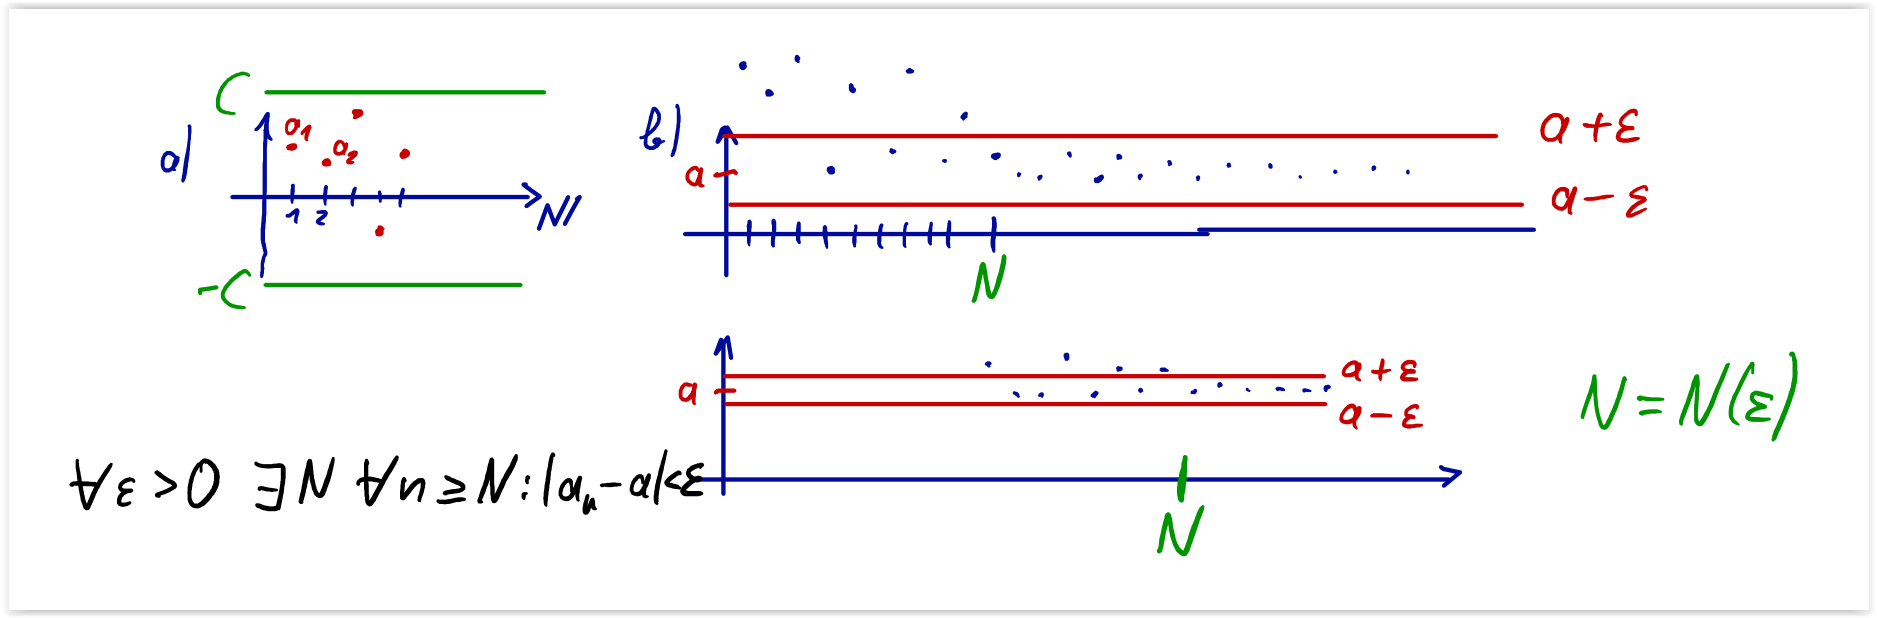
\includegraphics[width=0.9\textwidth]{./img/folge_epsil_krit.png}
	  \caption{Epsilon Kriterium\protect\cite{HM12}}
	  \label{fig:folge_epsilon}
	\end{figure}
  \begin{bem}
    Konvergiert $(a_n)_{n \in \N}$ gegen $a$ schreibt man
    \begin{align}
      &\lim_{n \rightarrow \infty} a_n = a\\
      &bzw. \nonumber \\
      &a_n \underset{n \rightarrow \infty}{\rightarrow} a \nonumber
    \end{align}
  \end{bem}
  \begin{bem}
    Die Schranke $N$ ist i.A. von $\varepsilon$ abhängig. Daher schreibt man $N(\varepsilon)$.
  \end{bem}
  \begin{bem}
    Der Grenzwert einer Folge ist eindeutig.
  \end{bem}
  
  \subsection{Ausdrücke mit Brüchen}
  $(a_n)$ mit $a_n = \frac{P(n)}{Q(n)}$ mit $P,Q$ sind Polynome.
  \begin{align*}
    \textbf{(1)}\quad grad(P) > grad(Q) &\Rightarrow (a_n) \text{ divergiert} \\
    \textbf{(2)}\quad grad(P) < grad(Q) &\Rightarrow (a_n) \text{ konvergiert gegen } 0\\
    \textbf{(3)}\quad grad(P) = grad(Q) &\Rightarrow (a_n) \text{ konvergiert gegen Quotient der Leitkoeffizienten}
  \end{align*}   
  
  \subsection{Dreiecksungleichung}
  \begin{align}
    |x+y| &\leq |x| + |y| \qquad ,\; x,y \in \R \\
    \text{bzw. in umgekehrter Form} \nonumber \\
    \big| |x| - |y| \big| &\leq |x-y|
  \end{align}
  
  \subsection{Beschränktheit}
  \begin{satz}
    Eine konvergente reelle Folge ist beschränkt.
  \end{satz}
  \begin{figure}[H] 
	  \centering
	  
\includegraphics[width=0.3\textwidth]{./img/beschraenkt.jpg}
	  \caption{derp derp derp}
	  \label{fig:folge_epsilon}
	\end{figure}
  
  \subsection{Grenzwertsätze}
  \begin{satz}
    Seien $(a_n)$, $(b_n)$ konvergente Folgen. Dann konvergieren auch die Folgen $\big(|a_n|\big)$, $(a_n + b_n)$ und $(\lambda a_n)$ für $\lambda \in \R$, und es gilt:
    \begin{itemize}
      \item[i) ] ~\\[-28pt]
      \begin{equation}
        \lim|a_n| = |\lim a_n|
      \end{equation}
      \item[ii) ] ~\\[-28pt]
      \begin{equation}
        \lim (a_n \pm b_n) = \lim a_n \pm \lim b_n
      \end{equation}       
      \item[iii) ] ~\\[-28pt]
      \begin{equation}
        lim (\lambda a_n) = \lambda \lim a_n
      \end{equation}
    \end{itemize}
  \end{satz}
  \begin{satz}
    Seien $(a_n)$, $(b_n)$ konvergente Folgen.
    \begin{itemize}
      \item[iv) ] Dann konvergiert auch $(a_n b_n)$ und es gilt\newline
      \begin{equation}
        lim (a_n b_n) = (\lim a_n)(\lim b_n)
      \end{equation}
      \item[v) ] Ist $b_n \neq 0$ für alle $n \in \N$ und $b \neq 0$, so konvergiert auch $\left( \frac{a_n}{b_n} \right)$ mit
      \begin{equation}
        \lim \left( \frac{a_n}{b_n} \right) = \frac{\lim a_n}{\lim b_n}
      \end{equation}
      \item[vi) ] Sei $m \in \N$. Ist $a_n \geq 0$ für alle $n \in \N$, dann konvergiert auch $\big( \sqrt[m]{a_n}\big)$ und es gilt
      \begin{equation}
        \lim \sqrt[m]{a_n} = \sqrt[m]{\lim a_n}
      \end{equation}
    \end{itemize}
  \end{satz}
  \begin{bem}
    Bei rationalen Ausdrücken mit der höchsten Potenz durchkürzen. Beispiel:
    \begin{equation*}
      \frac{n}{n^2+4n+8} = \frac{\frac{1}{n}}{1+\frac{4}{n}+\frac{8}{n^2}} \rightarrow \frac{0}{1}=0
    \end{equation*}
  \end{bem}
  
	  \subsubsection{Beispiele wichtiger Grenzwerte}
	  \begin{itemize}
	    \item[1) ] $\lim \frac{1}{n} = 0$
	    \item[2) ] Sei $q \in \R$ mit $|q| < 1$:\newline
	      $\lim q^n = 0$
	    \item[3) ] Sei $q \in \R$ mit $|q| < 1$ und $p \in \Z$:\newline
	      $\lim n^p q^n = 0$
	    \item[4) ] Sei $a \in \R$:\newline
	      $\lim \frac{a^n}{n!} = 0$
	    \item[5) ] $\;$\newline
	      $\lim\limits_{n \rightarrow \infty} \frac{n^k}{a^n} = 0$
	    \item[6) ] $\;$\newline
	      $\lim\limits_{n \rightarrow \infty} \sqrt[n]{c} = 1$
	    \item[7) ] $\;$\newline
	      $\lim\limits_{n \rightarrow \infty} \sqrt[n]{n} = 1$
	  \end{itemize}
	  
	\subsection{Konvergenzsätze}
	\begin{satz} $\;$\newline
	  \begin{itemize}
	    \item[1) ] Der Grenzwert einer konvergenten Folge ist eindeutig.
	    \item[2) ] Jede konvergente Folge ist beschränkt.
	    \item[3) ] Jede monotone und beschränkte Folge ist konvergent.
	      \begin{itemize}
	        \item[a) ]$(a_n)$ ist monoton wachsend und nach oben beschränkt 
	        \begin{equation*}
	          \Rightarrow \lim\limits_{n \rightarrow \infty} a_n = \sup\limits_{n \in \N} (a_n)
	        \end{equation*}
	        \item[b) ]$(a_n)$ ist monoton fallend und nach unten beschränkt 
	        \begin{equation*}
	          \Rightarrow \lim\limits_{n \rightarrow \infty} a_n = \inf\limits_{n \in \N} (a_n)
	        \end{equation*}
	      \end{itemize}
	  \end{itemize}
  \end{satz}  
  
  \subsection{Monotene Folgen}
  \begin{definition}
    Eine reelle Folge $(a_n)_{n \in \N}$ heißt monoton wachsend, falls $a_n \leq a_{n+1}$ für alle $n \in \N$. Sie heißt streng monoton wachsend, falls $a_n < a_{n+1}$ für alle $n \in \N$. Analog monoton fallend und streng monoton fallend.
  \end{definition}
  \begin{satz}
    Ist die Folge $(a_n)_{n \in \N}$ monoton wachsend und nach oben beschränkt, so konvergiert die Folge und es gilt
    \begin{equation}
      \lim_{n\rightarrow \infty} a_n = \sup \lbrace a_n : n\in \N \rbrace
    \end{equation}
  \end{satz}
  \begin{figure}[htbp] 
	  \centering
	  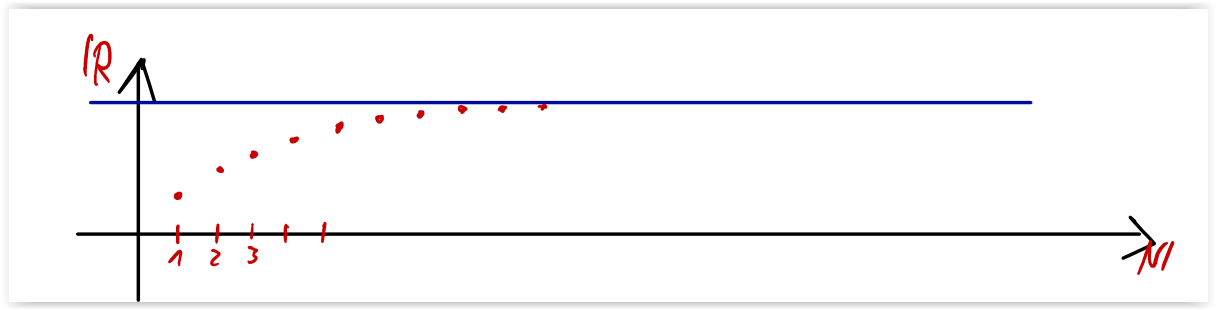
\includegraphics[width=0.9\textwidth]{./img/folge_monoton_beschraenkt.png}
	  \caption{Konvergenz mw u. beschr. Folgen\protect\cite{HM12}}
	  \label{fig:folge_mw_beschr}
	\end{figure}
	
		\subsubsection{Intervallschachtelung}
		Es seien $(a_n)_{n \in \N}$ und $(b_n)_{n \in \N}$ reelle Folgen.
		$(a_n)_{n \in \N}$ sei monoton wachsend und $(b_n)_{n \in \N}$ sei monoton fallend. Es gelte $(a_n)_{n \in \N} \leq (b_n)_{n \in \N}$ für alle $n \in \N$.
    Dann gilt 
    \begin{equation*}
      \lim_{n \rightarrow \infty} a_n,\quad \lim_{n \rightarrow \infty} b_n \quad ex.
    \end{equation*}
    und
    \begin{equation}
      \lim_{n \rightarrow \infty} (b_n - a_n) = 0 \Rightarrow \lim_{n \rightarrow \infty} a_n = \lim_{n \rightarrow \infty} b_n
    \end{equation}
\newpage
